 \documentclass[answers]{exam}
\usepackage{texPreamble}
\usepackage{relsize}
\usepackage{tabularx}
\extraheadheight{0.25in}
\extrafootheight{1.0in}
\extrawidth{1in}
% ----------------------------------------------------------------
\makeatletter
\title{Fall 2018 Class notes}
\author{\thefname\ \thelname}

\pagestyle{headandfoot}

\firstpageheader{\@title\\\@date}{}{Math 1040}
\firstpageheadrule

\newcommand{\currentname}{\@currentlabelname}

\runningfootrule
\runningfooter{\currentname}{\thepage}{\@title}
\makeatother
\begin{document}
%\relscale{1.4}
\section{JIT 6.1: The Family of Exponential Functions}
  \begin{defn*}
    An \textbf{exponential function} has the form $f(x)=a^x$, where $a>0$. The number $a$ is called the \textbf{base}.
  \end{defn*}
  \begin{ex*}\ 
  
    \noindent
    \begin{minipage}{0.5\linewidth}
      \begin{center}
        \begin{tabular}{@{}R@{\hspace*{35pt}}L@{\ =\,}L@{}}\toprule
          x& \multicolumn{2}{C}{f(x)}\\\midrule
          -1& 2\inv&\sfrac12\\
          0& 2^0&1\\
          \sfrac12& 2^{\sfrac{1}{2}}&\sqrt2\\
          2& 2^2&4\\
          3.2& 2^3\cdot2^{\sfrac{1}{5}}&8\sqrt[5]{2}\\\bottomrule
        \end{tabular}
      \end{center}
    \end{minipage}%
    \begin{minipage}{0.5\linewidth}
      \begin{center}
        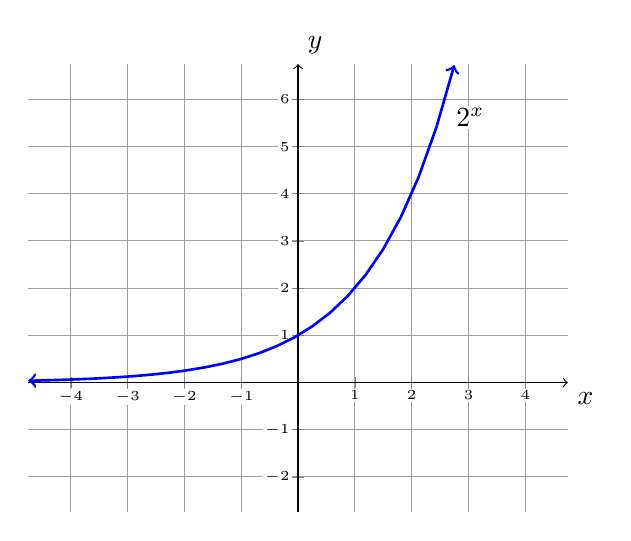
\begin{tikzpicture}
          \begin{axis}[
            grid=both,
            grid style={line width=0.35pt, draw=gray!75},
            axis lines=center,
            axis line style={->},
            xmin=-4, xmax=4,
            ymin=-2, ymax=6,
            xtick={-4,-3,...,4},
            ytick={-2,-1,...,6},
            enlargelimits={abs=0.75},
            ticklabel style={font=\tiny, inner sep=0.75pt,fill=white},
            xlabel=$x$, xlabel style={at={(ticklabel* cs:1)},anchor=north west},
            ylabel=$y$, ylabel style={at={(ticklabel* cs:1)},anchor=south west},
            every axis plot/.append style={line width=0.95pt}
            ]
            \addplot[<->] expression[domain=-4.75:2.75, blue] {2^x} node[inner sep=0.75pt, right, black, fill=white, pos=0.9, xshift=5pt] {$2^x$};
          \end{axis}
        \end{tikzpicture}
      \end{center}
    \end{minipage}%
  \end{ex*}
  \vfill
  The base $a$ determines if $a^x$ increases with exponential growth or decreases with exponential decay:
  
  \noindent
  \begin{minipage}{0.5\linewidth}
    \begin{center}
      $$a>1$$
      
        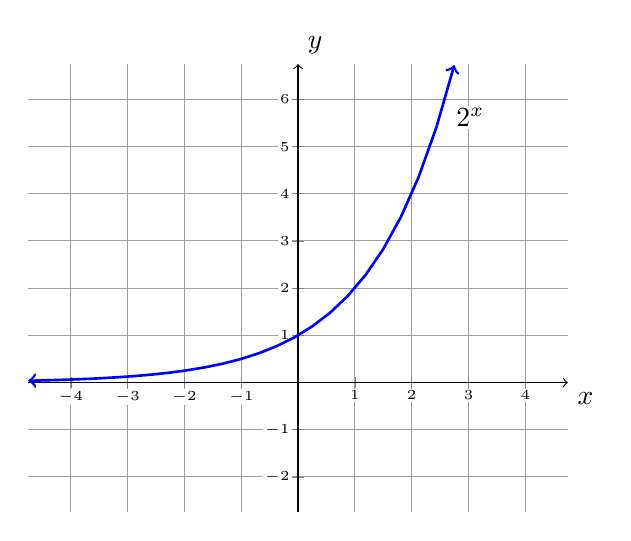
\begin{tikzpicture}
          \begin{axis}[
            grid=both,
            grid style={line width=0.35pt, draw=gray!75},
            axis lines=center,
            axis line style={->},
            xmin=-4, xmax=4,
            ymin=-2, ymax=6,
            xtick={-4,-3,...,4},
            ytick={-2,-1,...,6},
            enlargelimits={abs=0.75},
            ticklabel style={font=\tiny, inner sep=0.75pt,fill=white},
            xlabel=$x$, xlabel style={at={(ticklabel* cs:1)},anchor=north west},
            ylabel=$y$, ylabel style={at={(ticklabel* cs:1)},anchor=south west},
            every axis plot/.append style={line width=0.95pt}
            ]
            \addplot[<->] expression[domain=-4.75:2.75, blue] {2^x} node[inner sep=0.75pt,right, black, fill=white, pos=0.9, xshift=5pt] {$2^x$};
          \end{axis}
        \end{tikzpicture}
      \end{center}
  \end{minipage}%
  \begin{minipage}{0.5\linewidth}
    \begin{center}
      $$0<a<1$$
      
        \begin{tikzpicture}
          \begin{axis}[
            grid=both,
            grid style={line width=0.35pt, draw=gray!75},
            axis lines=center,
            axis line style={->},
            xmin=-4, xmax=4,
            ymin=-2, ymax=6,
            xtick={-4,-3,...,4},
            ytick={-2,-1,...,6},
            enlargelimits={abs=0.75},
            ticklabel style={font=\tiny, inner sep=0.75pt,fill=white},
            xlabel=$x$, xlabel style={at={(ticklabel* cs:1)},anchor=north west},
            ylabel=$y$, ylabel style={at={(ticklabel* cs:1)},anchor=south west},
            every axis plot/.append style={line width=0.95pt}
            ]
            \addplot[<->] expression[domain=-2.75:4.75, blue] {0.5^x} node[inner sep=0.75pt,left, black, fill=white, pos=0.1, xshift=-5pt] {$\sfrac{1}{2}^x$};
          \end{axis}
        \end{tikzpicture}
      \end{center}
  \end{minipage}%
  \pagebreak
  
  \begin{ex*}
    Graph $3^x$ and $5^x$ on the axes provided below:
    \begin{center}
      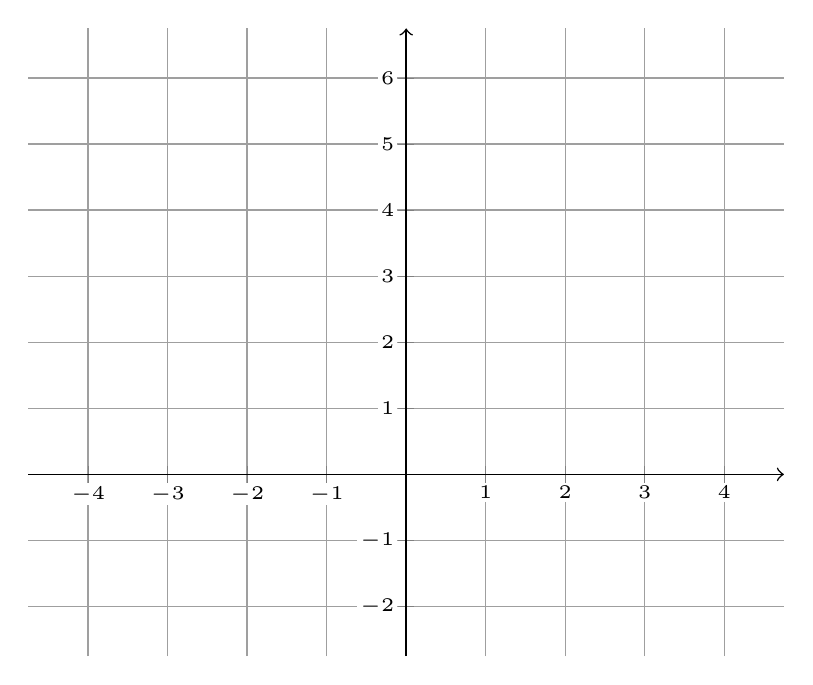
\begin{tikzpicture}[scale=1.4]
        \begin{axis}[
          grid=both,
          grid style={line width=0.35pt, draw=gray!75},
          axis lines=center,
          axis line style={->},
          xmin=-4, xmax=4,
          ymin=-2, ymax=6,
          xtick={-4,-3,...,4},
          ytick={-2,-1,...,6},
          enlargelimits={abs=0.75},
          ticklabel style={font=\tiny, inner sep=0.75pt,fill=white},
          every axis plot/.append style={line width=0.95pt}
          ]
        \end{axis}
      \end{tikzpicture}
    \end{center}
  \end{ex*}
  
  \vspace*{\stretch{1}}
  \begin{ex*}
    Graph $\parens{\dfrac{1}{3}}^x$ and $\parens{\dfrac{1}{5}}^x$ on the axes provided below:
    \begin{center}
      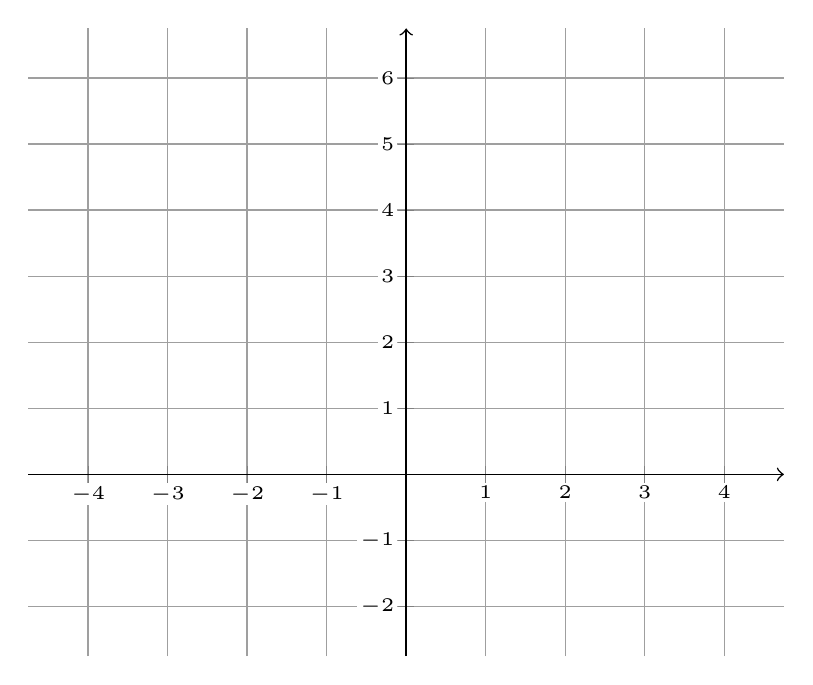
\begin{tikzpicture}[scale=1.4]
        \begin{axis}[
          grid=both,
          grid style={line width=0.35pt, draw=gray!75},
          axis lines=center,
          axis line style={->},
          xmin=-4, xmax=4,
          ymin=-2, ymax=6,
          xtick={-4,-3,...,4},
          ytick={-2,-1,...,6},
          enlargelimits={abs=0.75},
          ticklabel style={font=\tiny, inner sep=0.75pt,fill=white},
          every axis plot/.append style={line width=0.95pt}
          ]
        \end{axis}
      \end{tikzpicture}
    \end{center}
  \end{ex*}
  
  \pagebreak
  \begin{ex*}
    Graph $\parens{\dfrac{6}{7}}^x$ and $\parens{\dfrac{7}{6}}^x$:
    \begin{center}
      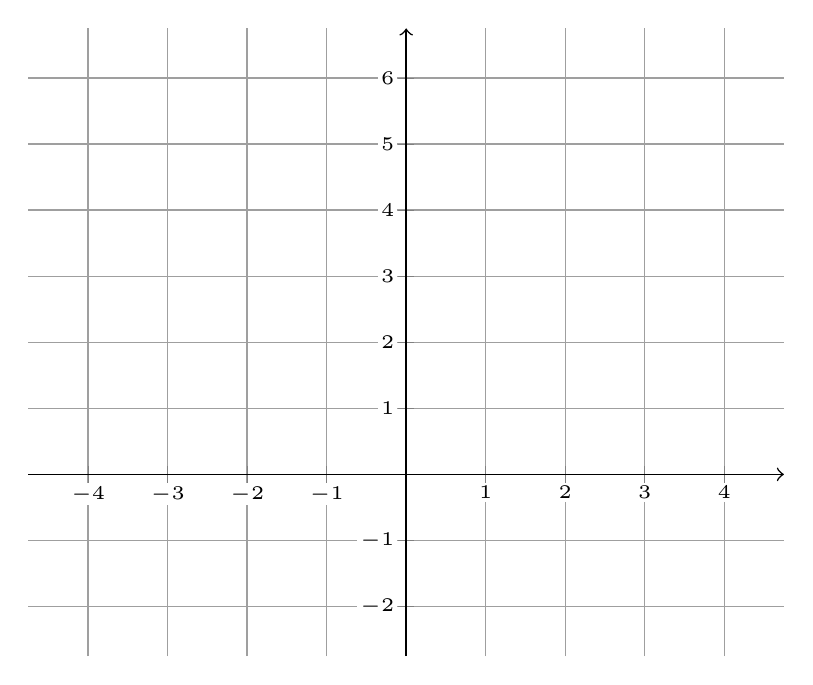
\begin{tikzpicture}[scale=1.4]
        \begin{axis}[
          grid=both,
          grid style={line width=0.35pt, draw=gray!75},
          axis lines=center,
          axis line style={->},
          xmin=-4, xmax=4,
          ymin=-2, ymax=6,
          xtick={-4,-3,...,4},
          ytick={-2,-1,...,6},
          enlargelimits={abs=0.75},
          ticklabel style={font=\tiny, inner sep=0.75pt,fill=white},
          every axis plot/.append style={line width=0.95pt}
          ]
        \end{axis}
      \end{tikzpicture}
    \end{center}
  \end{ex*}
  \vspace*{\stretch{1}}
  
\section{JIT 6.2: The Function $e^x$}
  \currentname
  
  The number $e$ is an irrational number whose exact form is
    $$e=\lim_{n \to \infty}\parens{1+\dfrac{1}{n}}^n\approx2.718281828459045\dots$$
    $$e^x=1+x+\frac{x^2}{2!}+\frac{x^3}{3!}+\frac{x^4}{4!}+\dots=\sum\nto[0]^\infty \dfrac{x^n}{n!}$$
  This exponential function has a $45^\circ$ tangent at $x=0$. This function shows in many applications, and each function $a^x$ can be written as $e^{kx}$.
  
  \pagebreak
  
  \begin{ex*}
    Graph $2^x, e^x$ and $3^x$:
  \end{ex*}
  \begin{center}
    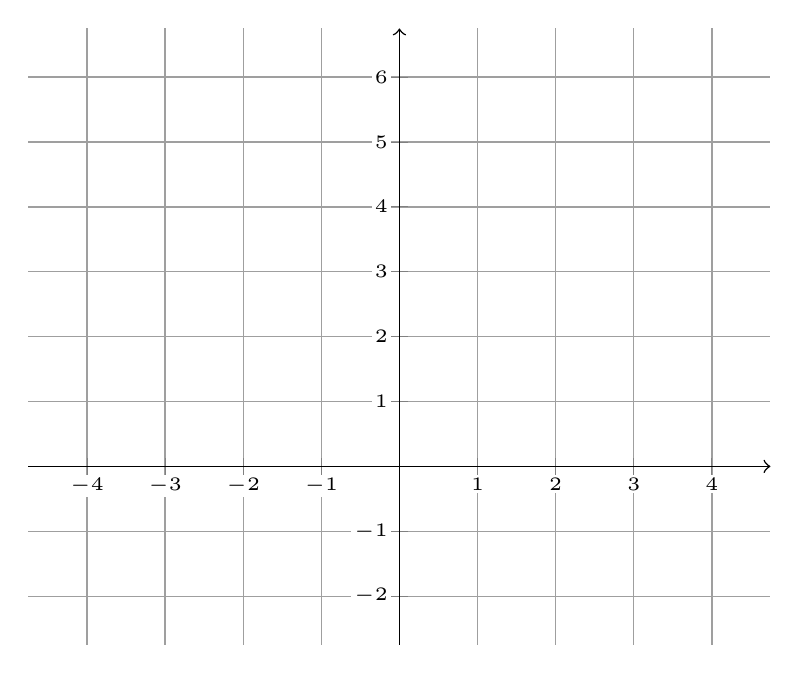
\begin{tikzpicture}[scale=1.375]
      \begin{axis}[
        grid=both,
        grid style={line width=0.35pt, draw=gray!75},
        axis lines=center,
        axis line style={->},
        xmin=-4, xmax=4,
        ymin=-2, ymax=6,
        xtick={-4,-3,...,4},
        ytick={-2,-1,...,6},
        enlargelimits={abs=0.75},
        ticklabel style={font=\tiny, inner sep=0.75pt,fill=white},
        every axis plot/.append style={line width=0.95pt}
        ]
      \end{axis}
    \end{tikzpicture}
  \end{center}
  \vspace*{\stretch{1}}

  \noindent
  All exponential functions follow the all the typical rules when performing transformation of functions:
  \begin{ex*}
    Graph $y=3^x,\ y=3^{x-1},\ y=3^{x+3},\ y=3^x+2,\ y=-3^x,\ y=3\inv[x]$
  \end{ex*}
  \begin{center}
    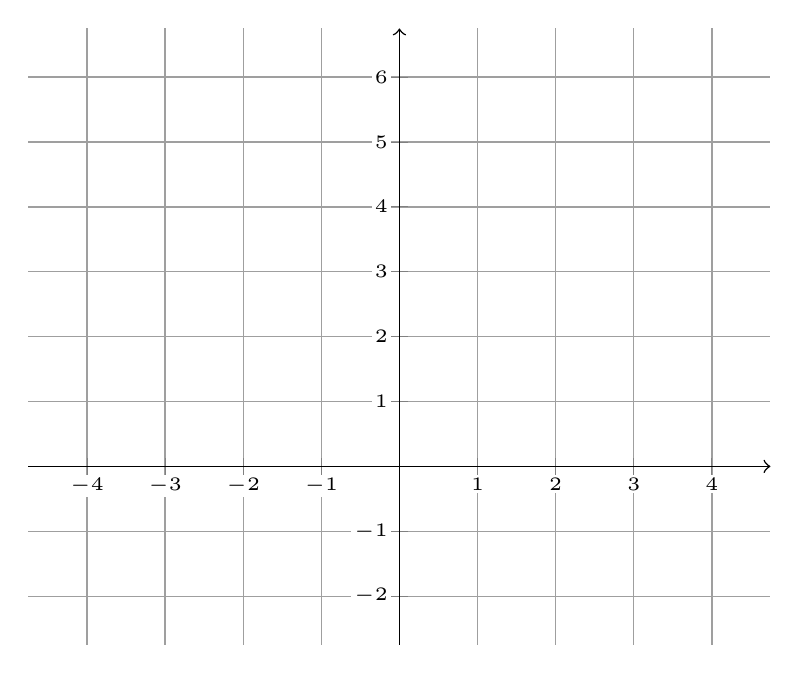
\begin{tikzpicture}[scale=1.375]
      \begin{axis}[
        grid=both,
        grid style={line width=0.35pt, draw=gray!75},
        axis lines=center,
        axis line style={->},
        xmin=-4, xmax=4,
        ymin=-2, ymax=6,
        xtick={-4,-3,...,4},
        ytick={-2,-1,...,6},
        enlargelimits={abs=0.75},
        ticklabel style={font=\tiny, inner sep=0.75pt,fill=white},
        every axis plot/.append style={line width=0.95pt}
        ]
      \end{axis}
    \end{tikzpicture}
  \end{center}

  
  \pagebreak
  \begin{ex*}\ 
  
  \noindent
  \begin{minipage}[t]{0.625\linewidth}
    
    Solve:
    \begin{tasks}[after-item-skip=0.125\paperheight](1)
      \task $2^{x-3}=64$
      \task $4^{2x-3}=64$
    \end{tasks}
  \end{minipage}%
  \begin{minipage}[t]{0.375\linewidth}\ 
  
    \flushright
    \fbox{\parbox{0.85\linewidth}{
    \underline{Properties of exponents}
    \begin{enumerate}
      \item $a^m\cdot a^n=a^{m+n}$
      \item $\dfrac{a^m}{a^n}=a^{m-n}$
      \item $\parens{a^m}^n=a^{mn}$
      \item $\parens{ab}^n=a^nb^n$
      \item $\parens{\dfrac{a}{b}}^n=\dfrac{a^n}{b^n}, b\neq 0$
      \item $a\inv[n]=\frac{1}{a^n}, a\neq 0$
      \item $a^0=1, a\neq 0$
    \end{enumerate}
  }}
  \end{minipage}%
  \begin{tasks}[resume, after-item-skip=0.075\paperheight](3)
    \task $10^{\sin x}=1$
    \task $5^{x^2+2x}=125$
    \task $\parens{\dfrac{1}{4}}^{2-x}=16^x$
  \end{tasks}
  \end{ex*}
  \vspace*{\stretch{1}}
  
  \begin{ex*}
    Simplify:
    \begin{tasks}(3)
      \task $\parens{e^x}^3$
      \task $\dfrac{e^{2x}}{e^x}$
      \task $\dfrac{e^{2x}-1}{e^x-1}$
    \end{tasks}
  \end{ex*}
  \vspace*{\stretch{1}}
  
  \pagebreak
  
  \section{JIT 7.1: Composition and Inverse Functions}
  
  \begin{defn*}
    Given two functions $f$ and $g$, the composite function $f\circ g$ is defined by $(f\circ g)(x)=f\parens{g(x)}$. It is evaluated in two steps: $y=f(u)$, where $u=g(x)$. The domain of $f\circ g$ consists of all $x$ in the domain of $g$ such that $u=g(x)$ is in the domain of $f$.
  \end{defn*}
  \begin{ex*}
    Given $f(x)=x^2+2x+\pi$ and $g(x)=x^2$, find
    \begin{itemize}[label=, itemsep=\stretch{1}]
      \item $f\parens{g(x)}$
      \item $g\parens{f(x)}$
    \end{itemize}
  \end{ex*}
  \vspace*{\stretch{1}}
  \begin{ex*}
    Given $f(x)=\dfrac{1}{x+2}$ and $g(x)=x^2-1$, find
    \begin{itemize}[label=, itemsep=\stretch{1}]
      \item $f\parens{g(x)}$
      \item $g\parens{f(x)}$
    \end{itemize}
  \end{ex*}
  \vspace*{\stretch{1}}
  \begin{ex*}
    Given $f(x)=x^2, g(x)=\sin(x)$ and $h(x)=2x+1$, find 
    \begin{itemize}[label=, itemsep=\stretch{1}]
      \item $f(g(h(x)))$
    \end{itemize}
  \end{ex*}
  \vspace*{\stretch{1}}
  
  \pagebreak
  
  \begin{ex*}
    Given $f(x)=x^3, g(x)=\cos(x)$, find
    \begin{tasks}[after-item-skip=\stretch{1}](4)
      \task[] $f(0)$ 
      \task[] $f(1)$
      \task[] $g(0)$ 
      \task[] $(f\circ g)(0)$
      \task[] $(f\circ g)(x)$
      \task[] $(g\circ f)(x)$
      \task[] $(f\circ f)(x)$
      \task[] $(g\circ g)(x)$
    \end{tasks}
  \end{ex*}
  
  \vspace*{\stretch{1}}
  \begin{ex*}
    Evaluate or explain why the functions value is undefined:
  \end{ex*}
  \noindent
  \begin{minipage}[t]{0.5\linewidth}\ 
    
    \begin{enumerate}[label=,itemsep=15pt]
      \item $f\parens{g(2)}$
      \item $g\parens{f(2)}$
      \item $\parens{f\circ g}(0)$
      \item $\parens{g\circ f}(6)$
      \item $\parens{g\circ g}(-2)$
      \item $\parens{f\circ f}(4)$
    \end{enumerate}
    \vspace*{15pt}
  \end{minipage}%
  \begin{minipage}[t]{0.5\linewidth}\ 
  
    \begin{flushright}
      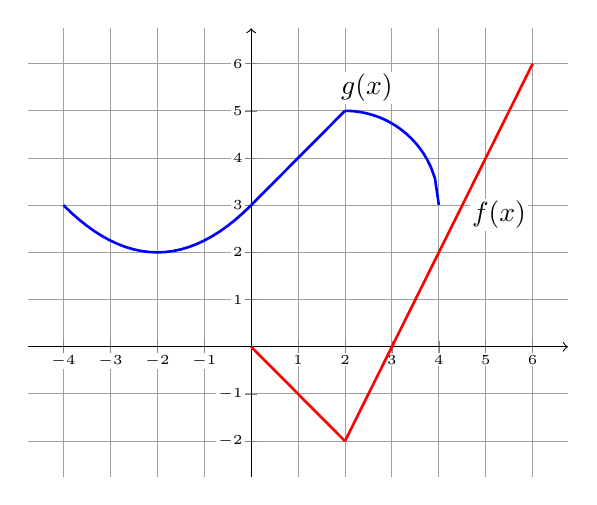
\begin{tikzpicture}
        \begin{axis}[
          grid=both,
          grid style={line width=0.35pt, draw=gray!75},
          axis lines=center,
          axis line style={->},
          xmin=-4, xmax=6,
          ymin=-2, ymax=6,
          xtick={-4,-3,...,6},
          ytick={-2,-1,...,6},
          enlargelimits={abs=0.75},
          ticklabel style={font=\tiny, inner sep=0.75pt,fill=white},
          every axis plot/.append style={line width=0.95pt}
          ]
          \addplot[-] expression[domain=-4:0, blue] {(0.5*(x+2))^2+2};
          \addplot[-] expression[domain=0:2, blue] {x+3};
          \addplot[-] expression[domain=2:4, blue] {sqrt(4-(x-2)^2)+3} node[inner sep=0.75pt, above, black, pos=0.15, fill=white, yshift=3pt] {$g(x)$};
          %
          \addplot[-] expression[domain=0:2, red] {-x};
          \addplot[-] expression[domain=2:6, red] {2*x-6} node[inner sep=0.75pt, right, black, pos=0.6, fill=white, xshift=4pt] {$f(x)$};
        \end{axis}
      \end{tikzpicture}
    \end{flushright}
  \end{minipage}
  \begin{description}
    \item[Note:] $f\parens{g(x)}$ is not necessarily the same as $g\parens{f(x)}$.
    \item[Note:] If $f\parens{g(x)}=x$ and $g\parens{f(x)}=x$, then $f(x)$ and $g(x)$ are inverse functions.
  \end{description}
  \pagebreak
  
\end{document}
